\documentclass{standalone}
\usepackage{tikz}
\usetikzlibrary{shapes.geometric,arrows}
\usetikzlibrary{fit}
\usetikzlibrary{backgrounds} 

\tikzstyle{startstop} = [rectangle, rounded corners, minimum width=3cm, minimum height=1cm, text centered, draw=black, fill=red!30]
\tikzstyle{io}        = [trapezium, trapezium left angle=70, trapezium right angle=110, minimum width=3cm, inner xsep = -15pt, minimum height=1cm, text centered, draw=black, fill=blue!30]
\tikzstyle{process}   = [rectangle, minimum width=3cm, minimum height=1cm, inner ysep=0, text centered, draw=black, fill=orange!30]
\tikzstyle{decision}  = [diamond,shape aspect=2.5, minimum width=3cm, minimum height=1cm, inner xsep=0,text centered, draw=black, fill=green!30]
\tikzstyle{arrow}     = [thick,->,>=stealth]

\begin{document}
  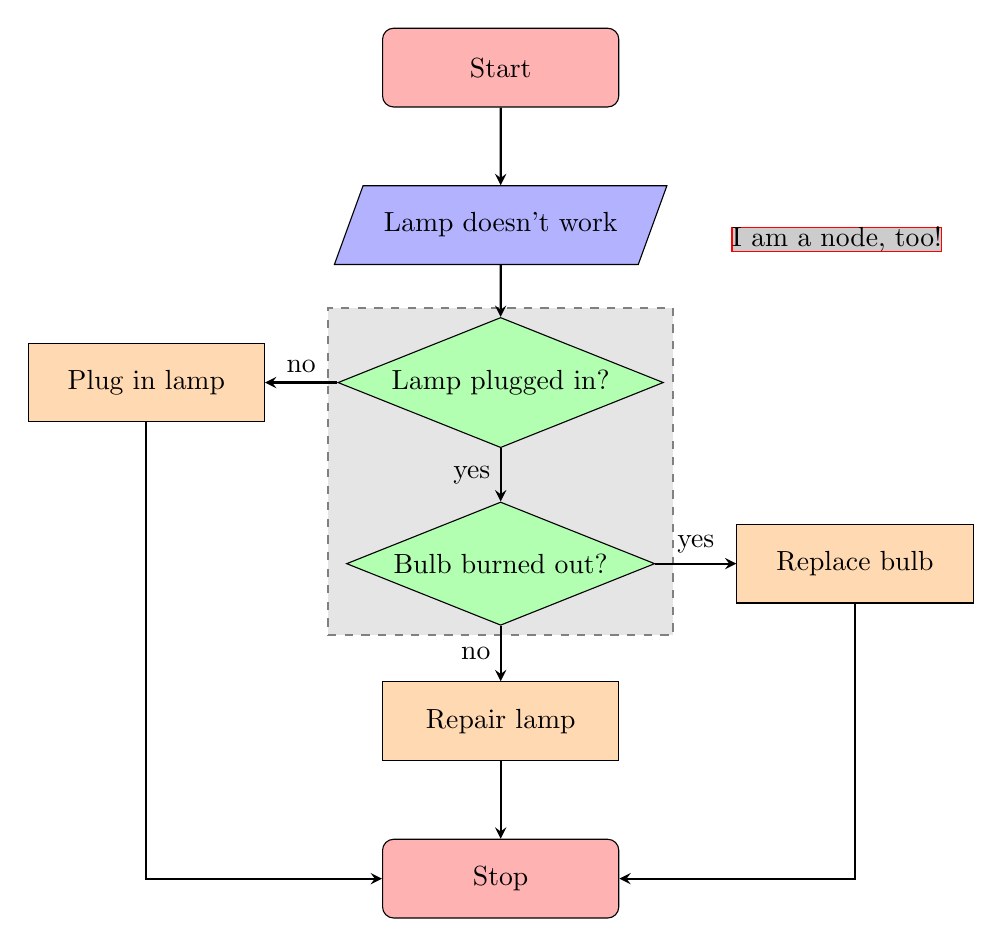
\begin{tikzpicture}[node distance=2cm]
    % adding nodes
    \node (start) [startstop] {Start};
    \node (io1)   [io, below of=start] {Lamp doesn't work};
    \node (dec1)  [decision, below of=io1] {Lamp plugged in?};
    \node (dec2)  [decision, below of=dec1, yshift=-0.3cm] {Bulb burned out?};
    
    \node (pro2) [process, below of=dec2] {Repair lamp};
    \node (stop) [startstop, below of=pro2] {Stop};
    
    \node (pro3) [process, left of=dec1, xshift=-2.5cm] {Plug in lamp};
    \node (pro4) [process, right of=dec2, xshift=2.5cm] {Replace bulb};
    
    % adding frame
    \begin{scope}[on background layer,label distance=1cm] % if you prefer pin, pin distance=1cm, and change label below to pin
      \node [draw=black!50,dashed,thick,fill=black!10,fit=(dec1) (dec2),label={[draw=red,fill=black!20,inner sep=0,anchor=south west]north east:{I am a node, too!}}] {};
    \end{scope} 
  
    % adding arrows
    \draw [arrow] (start) -- (io1);
    \draw [arrow] (io1) -- (dec1);
    \draw [arrow] (dec1) -- node[anchor=east] {yes} (dec2);
    \draw [arrow] (dec2) -- node[anchor=east] {no } (pro2);
    
    \draw [arrow] (dec1) -- node[anchor=south] {no }(pro3);
    \draw [arrow] (dec2) -- node[anchor=south] {yes}(pro4);
    
    \draw [arrow] (pro4) |- (stop);
    \draw [arrow] (pro3) |- (stop);
    
    \draw [arrow] (pro2) -- (stop);
  \end{tikzpicture}

\end{document}
